\section{Introduction}

Smart contracts often utilize time values to trigger specific actions. The
values that can be employed for this purpose include the block timestamp and
the block number. However, under the Proof of Work (PoW) consensus mechanism in
Ethereum, using these values has been associated with various security issues
\cite{swc116} \cite{Conkas2021} \cite{DASP2018} \cite{Osiris2018}
\cite{Oyente2016}.


Since the transition to the Proof of Stake (PoS) consensus mechanism in
Ethereum, significant changes have occurred in how the timestamp value has to
be set and in the stability of the block time. This paper aims to discuss these
changes.

\section{Ethereum's Consensus Mechanisms}
Ethereum initially adopted the Proof of Work (PoW) mechanism, a process known
for its security and decentralization but also criticized for its high energy
consumption and potential for centralization due to mining pools. PoW requires
miners to solve complex computational problems to validate transactions and
create new blocks, a process that consumes substantial computational power and
energy \cite{eth_pow}.

In response to these concerns, Ethereum transitioned to the Proof of Stake
(PoS) mechanism with "The Merge" on September 15, 2022. PoS, in contrast to
PoW, selects validators to create new blocks based on the number of coins they
hold and are willing to 'stake' as collateral. This approach significantly
reduces the energy requirements and aims to offer a more scalable and
environmentally friendly alternative \cite{eth_merge}.


\section{Block Time in Ethereum}

\subsection{Proof-of-Work Block Time}
\label{diff_adjustment}

In Ethereum's Proof-of-Work (PoW) system, the block time — the average time
interval between blocks — is primarily governed by a difficulty adjustment
algorithm. This algorithm dynamically alters the computational difficulty of
mining a block, striving to keep the block time within a targeted range.
According to Ethereum Improvement Proposal 2 (EIP-2), the algorithm adjusts
difficulty levels based on observed block times \cite{eip-2}:

\begin{itemize}
  \item If the block time falls short of the ideal duration (less
    than 10 seconds), the difficulty is increased. This escalation in
    difficulty slows down the rate at which new blocks are mined,
    counteracting the tendency towards overly rapid block generation.

  \item Conversely, if the block time stretches beyond the desired limit (exceeding
    20 seconds), the difficulty is decreased. This reduction makes it easier to
    mine new blocks, compensating for excessively lengthy block intervals.
\end{itemize}


The following pie chart provides a graphical depiction of Ethereum's block time
distribution under the Proof of Work (PoW) mechanism for the year 2021,
highlighting significant fluctuations, with an average block time of
approximately 13.4 seconds.


\begin{figure}[H]
  \centering
  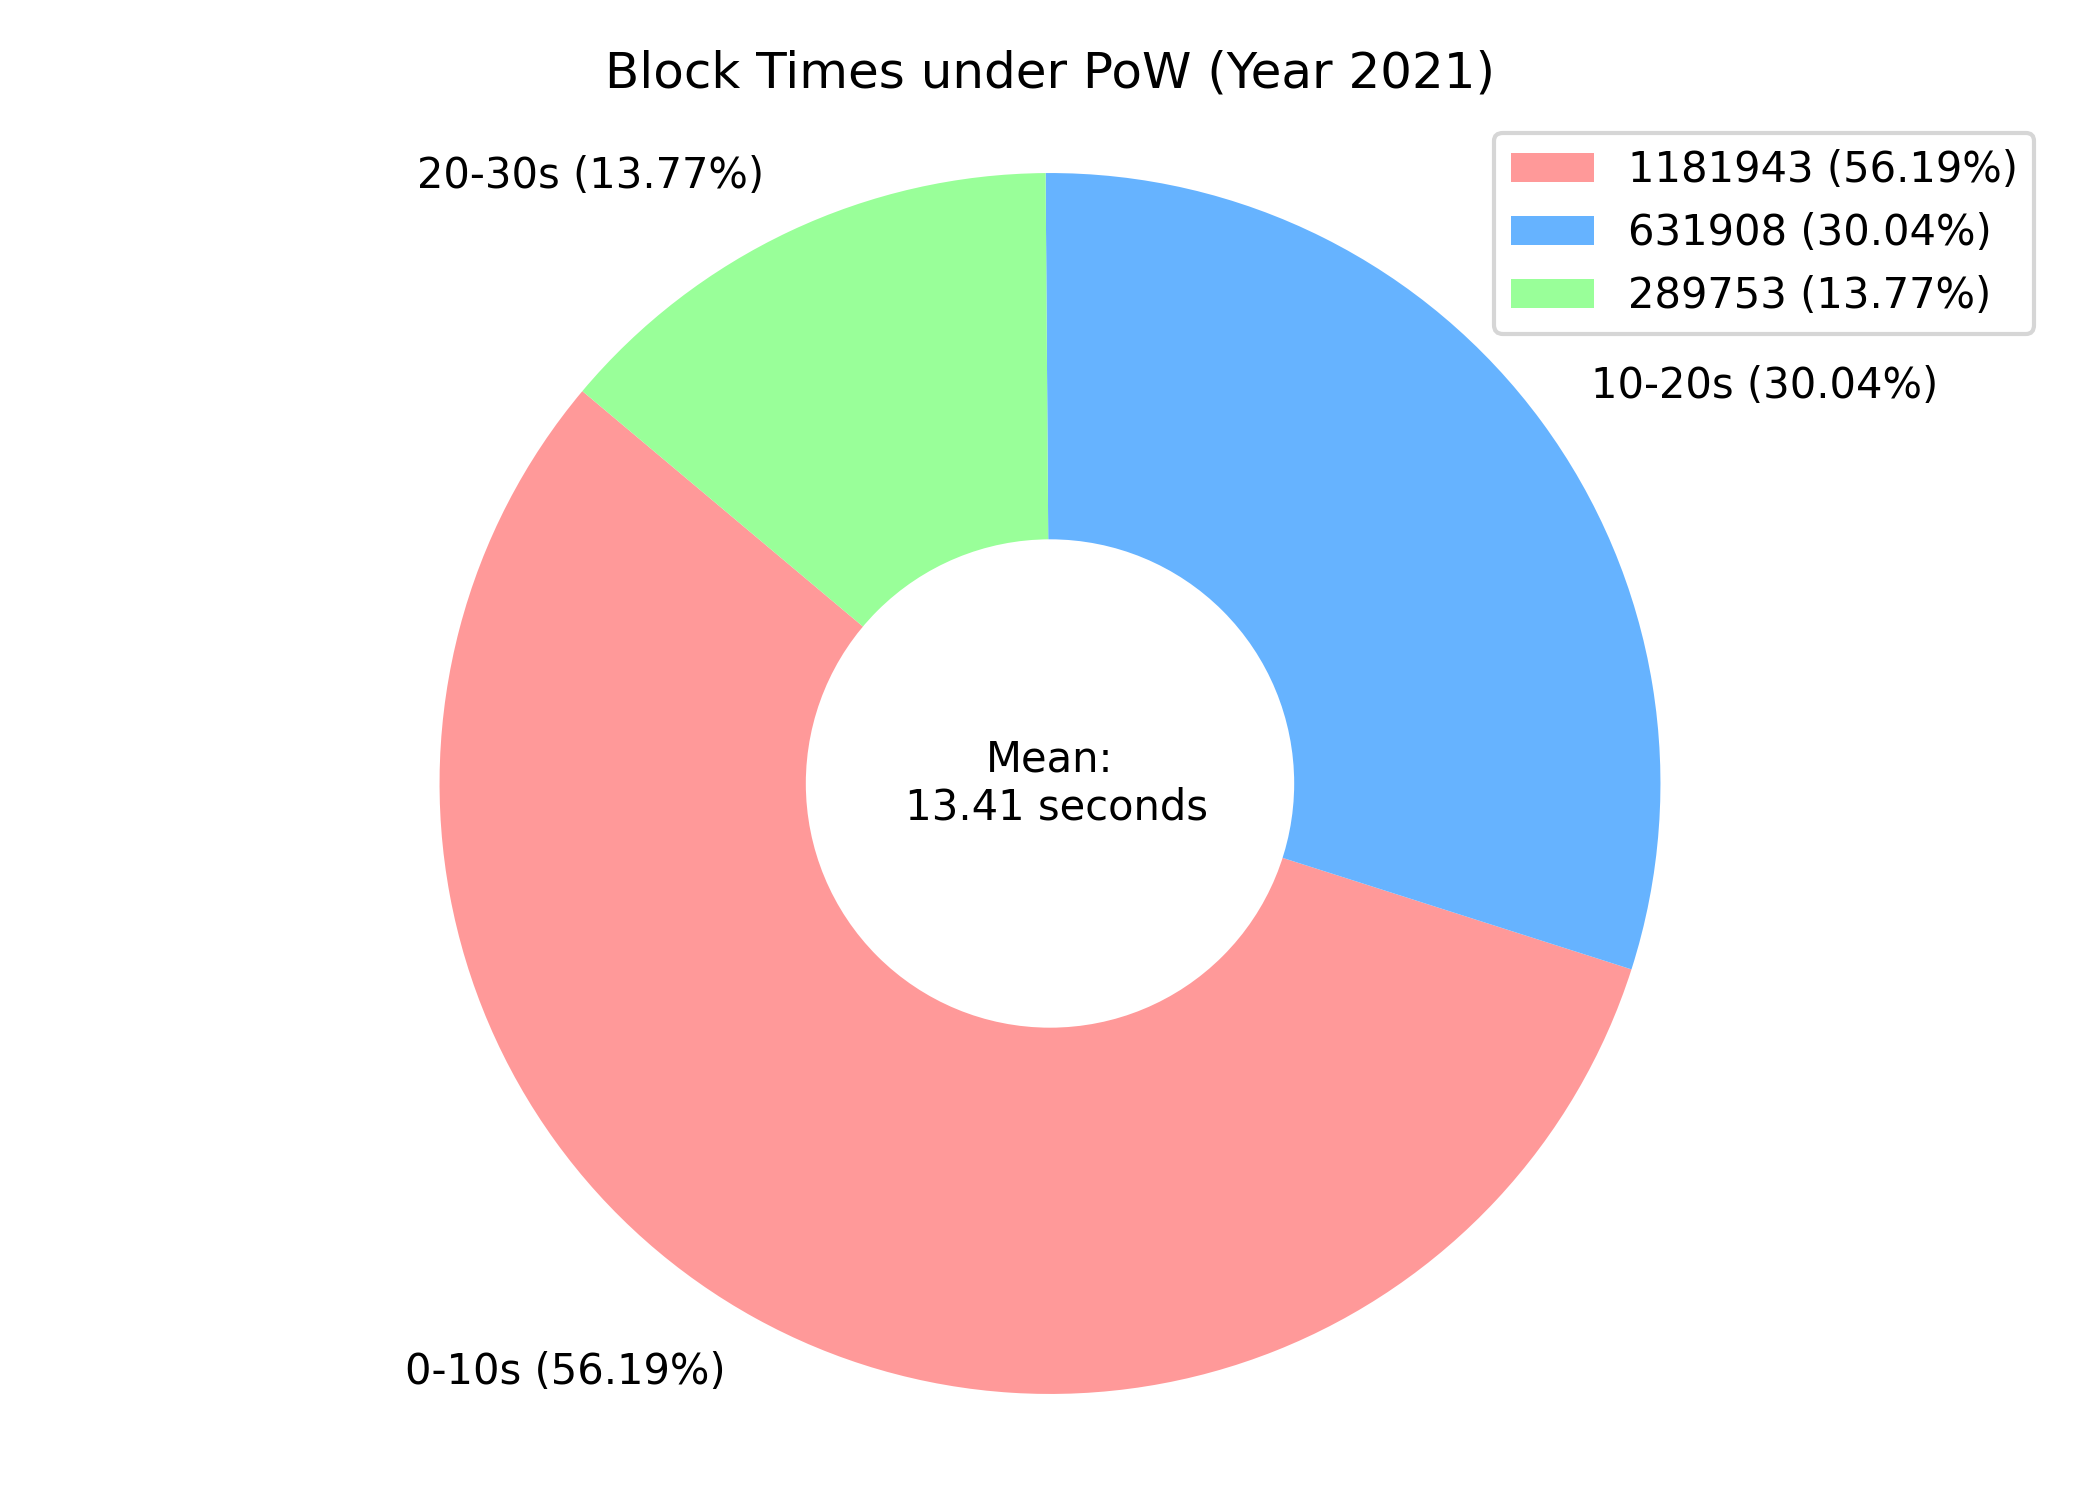
\includegraphics[width=0.8\textwidth]{block_time_analysis/pow_block_time_pie_chart.png}
  \caption{Block times under PoW in the year 2021.}
  \label{fig:block_time_analysis_pow}
\end{figure}

\subsection{Proof-of-Stake Block Time}
Following "The Merge" on September 15, 2022, Ethereum has shifted to a
Proof-of-Stake (PoS) consensus mechanism \cite{eth_history}. Under PoS, validators propose new
blocks, with a selection process involving other validators who vote to confirm
these blocks' authenticity. A stake of 32 ETH is required to be locked in as a
deposit for one to become a validator. This staking mechanism ensures validator
honesty, as any malpractice could lead to the loss of their staked ETH.

The PoS system is organized around slots and epochs, with slots being 12-second
intervals and an epoch consisting of 32 such slots
\cite{seconds-per-slot-mainnet}\cite{seconds-per-slot-mainnet-doc}. A validator
is chosen by
the protocol's algorithm to propose a block in each slot, and failure to comply
with the protocol's rules in block creation can result in their block being
dismissed. This structure introduces a more predictable and systematic approach
to block creation compared to PoW.

In the event that the selected validator, responsible for proposing a new block,
is offline, the slot remains empty \cite{validator-offline}. The timestamp of
the following block aligns with the timestamp of the following slot, which is a
multiple of 12 seconds. As a result, blocks are 24 seconds
apart. If subsequent validators are also offline, the block times will be 36
seconds apart, and so on.

An examination of the blockchain data since the implementation of the Merge
(starting at block number 15537393) reveals that 99.05\% of all blocks have been
consistent with a block time of 12 seconds, as indicated by the data in Figure
\ref{fig:block_time_analysis}.

\begin{figure}[H]
  \centering
  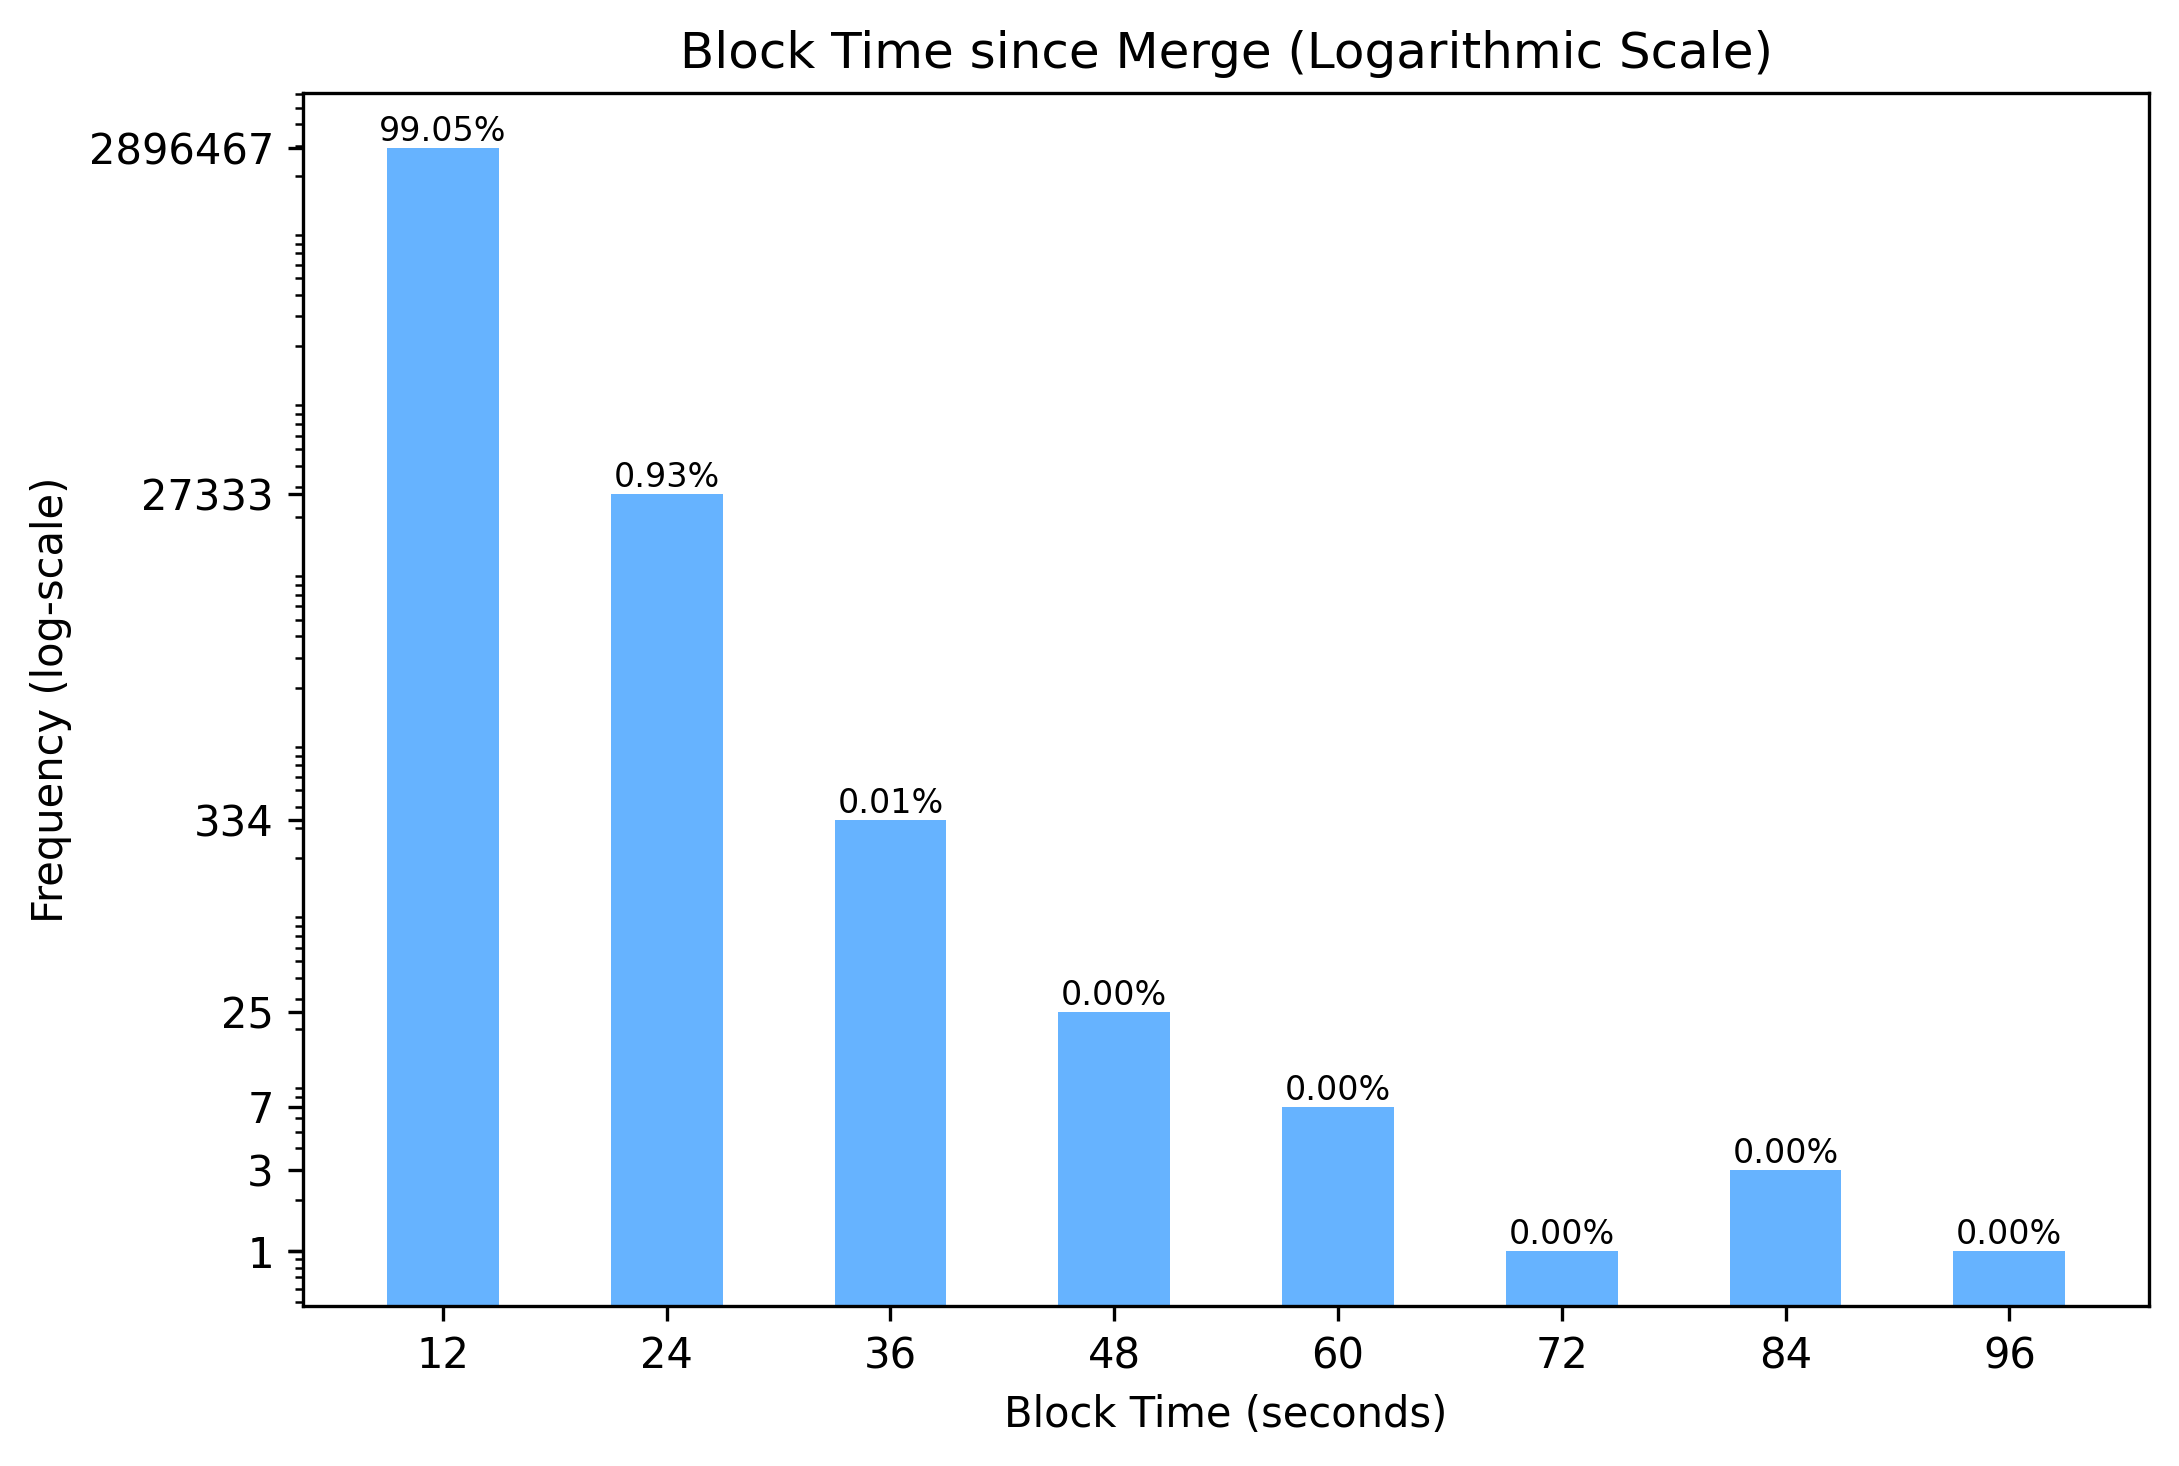
\includegraphics[width=1\textwidth]{block_time_analysis/pos_block_time_bar_chart_with_percentages.png}
  \caption{Block times since the merge.}
  \label{fig:block_time_analysis}
\end{figure}

\section{Block timestamp in Ethereum}
\subsection{Proof-of-Work Block Timestamp}
As discuessed in \ref{diff_adjustment} the block time had the
potential to vary from one block to another. Furthermore, the only restriction
miners had to follow when setting the block timestamp value was outlined in the
yellow paper, which stipulated that the timestamp of the new block must be
greater than the timestamp of the parent block \cite{ethyellowpaper2023}.
Consequently, miners could gain an unfair advantage by manipulating the
timestamp of their mined block \cite{swc116}.


To prevent miners from setting the timestamp too far into the future, some of the most widely used Ethereum implementations, such as Geth (go-ethereum), implemented a rejection mechanism for blocks with timestamps exceeding 15 seconds into the future \cite{go-ethereum-15-sek-limit}.

Hence, when the PoW consensus mechanism was in use, miners had the ability to
manipulate the timestamp and adjust it by up to 15 seconds. This behavior led
to the establishment of the "15-second Rule"
\footnote{\url{https://consensys.github.io/smart-contract-best-practices/development-recommendations/solidity-specific/timestamp-dependence/}},
as a security best practice. The
rule suggests that the usage of the block timestamp is considered
safe if the time-dependent event can tolerate a variation of up to 15 seconds.

\subsection{Proof-of-Stake Block Timestamp}

The PoS Ethereum consensus specification provides instructions on how to
calculate the timestamp at a specific slot using the
\textit{compute\_timestamp\_at\_slot} function \cite{compute-timestamp-at-slot}.
This calculation is based on the following formula:

\begin{equation}
genesis\_time + slots\_since\_genesis *
seconds\_per\_slot
\end{equation}


In the Ethereum mainnet configuration, the value of \textit{seconds\_per\_slot} is set to
12 seconds \cite{seconds-per-slot-mainnet} \cite{seconds-per-slot-mainnet-doc}.
The mainnet beacon chain's value for \textit{genesis\_time} is $1606824023$, which
corresponds to the timestamp when the original PoS beacon chain was launched on
December 1, 2020.

Each validator calculates the block timestamp in the same way and verifies if
the timestamp in the block matches the calculated timestamp. If there is a
mismatch, the block is rejected \cite{process-execution-payload}. Since each
slot, and consequently each block, has a predetermined timestamp, it is
virtually impossible to tamper with, but it also becomes more predictable.

\section{Block number in Ethereum}
\subsection{Proof-of-Work Block Number}
The yellow paper of Ethereum states that each block has
an integer value as a block number. The block number
of a specific block must be exactly one unit higher than the block
number of the previous block \cite{ethyellowpaper2023}.
Smart contract developers attempted to utilize the block number to calculate
the current time, operating under the assumption that the time interval between
two blocks always remains constant at fourteen seconds. Theoretically, one could
calculate time differences between blocks by multiplying the block numbers by fourteen 
and subtracting them from each other.
However, this approach proves impractical in reality due to the variable
intervals between blocks, as explained earlier. Moreover, these block intervals
can change unexpectedly, for instance, when the difficulty bomb was introduced
or during a chain fork \cite{swc116}.
As a result the block number should not be used as a proxy for time.
%An example for this misusage can be seen in the Listing \ref{lst:number_weakness}.
%There the block number is used to lock a function of a contract for a specific time.

%\lstinputlisting[language=Solidity, caption={Block Number Weakness in PoW},linerange={4-17}, label={lst:number_weakness}]{../dev/contracts/blocknumbertimelock.sol}

\subsection{Proof-of-Stake Block Number}
In PoS, just like in PoW, the block number increases by one with each new block.
In PoS, the block intervals are consistently set at 12 seconds.
Consequently, it might appear that using the block number as a time proxy in PoS is a viable option. 
However, it's not advisable, because validators go offline from time to time.
This causes the block time to increase and therefore leads to an inaccuracy of the calculation
of time based on the block number. \\
% (like the one in Listing \ref{lst:number_weakness})
A contract initially deployed under PoW would
become impractical or malfunction in a PoS environment due to the inherent differences in the block times.

\section{Conclusion: Block Time under PoW vs. PoS}
In PoW-based Ethereum, block times were probabilistic and influenced by mining difficulty.
As a result, using block values as a time proxy in PoW was not secure.
However, since Ethereum's transition to PoS, this is no longer the case.
PoS-based Ethereum has fixed block times of 12 seconds or multiples thereof.
Our research has shown that block times can no longer be influenced from external sources.
Therefore, using the block.timestamp value as a time proxy is now safe in PoS.

Using the block.number as a proxy for time is still not advisable. Block times 
can become a multiple of 12s and it is also not guaranteed that the block intervals will
never change again in the future.
